\documentclass[aps,prl,twocolumn,groupedaddress, reprint,floatfix,nofootinbib,longbibliography]{revtex4-2}
\usepackage{amsmath,amssymb,amsfonts}
\usepackage{bm}
\usepackage{graphicx}
\usepackage{hyperref}
\usepackage{braket}
\usepackage{color}
\usepackage{fontawesome}

\newcommand{\github}[1]{\href{#1}{\faGithubSquare}}
\newcommand{\esrgithub}{\github{https://github.com/MatthieuSarkis/https://github.com/MatthieuSarkis/magic_mol}}

\DeclareMathOperator*{\argmax}{argmax}

\begin{document}

    \title{Are molecules magical?\\[0.2em]
    \small Non-Stabilizerness in Molecular Bonding}
    \author{Matthieu Sarkis}
    \email[]{matthieu.sarkis@uni.lu}
    \affiliation{Department of Physics and Materials Science, University of Luxembourg, Luxembourg}
    \date{\today}

\begin{abstract}
    In this short note, we argue that the process of formation of bound states in molecular systems is characterized by a high degree of non-stabilizerness, as quantified by various magic proxies of the electronic ground state of the system. We illustrate this concept by studying the H$_2$ dimer as a prototypical system exhibiting bonding and show that the stabilizer Renyi entropy, a well-established magic monotone, exhibits a neat pick which is closely correlated to the binding energy curve of the system. We discuss possible implications of this observation.
\end{abstract}

\maketitle

\section{Introduction}

    Quantum entanglement is a fundamental feature of many-body physics and quantum chemistry, reflecting nonclassical correlations between constituents \cite{rissler2006measuring,boguslawski2015orbital,ding2025entanglement}. It has become a key diagnostic in a wide range of systems—from condensed matter to molecular bonds—often quantified by measures such as the von Neumann entropy or Rényi entropies of reduced density matrices \cite{szalay2017correlation}. For example, in molecular systems such as the hydrogen molecule H$_2$, entanglement between electrons is negligible when the atoms are far apart or nearly fused into a single nucleus, but grows as a covalent bond forms. However, it is now understood that entanglement alone is not a sufficient indicator of a quantum state’s computational complexity or \textit{quantumness} \cite{bravyi2005universal,howard2014contextuality}. There exist highly entangled yet classically simulable states, notably the so-called \textit{stabilizer states} that can be produced by Clifford gates—transformations belonging to the normalizer of the Pauli group—and efficiently simulated on a classical computer via the Gottesman-Knill theorem. In other words, entanglement by itself does not guarantee quantum advantage. The resource that elevates a quantum state beyond stabilizer dynamics is referred to as \textit{non-stabilizerness} or \textit{magic}, as described by the resource theory of stabilizer quantum computation \cite{howard2014contextuality}. Stabilizer states and Clifford operations are considered \textit{free} since they can be simulated efficiently on a classical computer, whereas non-stabilizer states provide the essential resource for transcending classical simulability. Magic can be quantified by various monotones that do not increase under stabilizer operations; one convenient measure is the \textit{mana}, defined via the negativity of the state’s discrete Wigner function \cite{howard2014contextuality}. Indeed, stabilizer states possess a positive Wigner function, and for pure states, mana vanishes if and only if the state is a stabilizer state—a discrete analog of Hudson’s theorem linking positive Wigner representations to Gaussian (stabilizer) states, thereby underlining that negativity in the quasiprobability distribution is essential for a state to supply quantum computational advantage. Besides mana, other magic measures have been proposed, such as the \textit{robustness of magic} \cite{howard2017application,heinrich2019robustness,hamaguchi2024handbook} and the \textit{stabilizer Rényi entropies} \cite{leone2022stabilizer}.

    To sum up, magic indicate the \textit{quantum overhead} inherent in accurately modeling a system. If a molecular system has low magic, then a classical method might suffice. High magic, on the other hand, flags the need for quantum computational resources. Our results on H$_2$ will illustrate this point: we will see that the region where H$_2$ coincides with a surge in mana, i.e. the emergence of strong magic in the wavefunction.

    In parallel, quantum information concepts have begun to permeate the study of molecules and chemical bonding. The process of bond formation is inherently quantum, involving superposition of atomic configurations and entanglement between electrons. Measures such as entanglement entropy have been used to characterize these correlations in chemical systems. Rissler, Noack, and White \cite{rissler2006measuring} applied quantum information theory in chemistry by introducing orbital mutual information as a measure of electron interactions between orbitals, a concept that not only successfully identifies chemical bond patterns but also aids in optimizing DMRG algorithms. Building on this foundation, Boguslawski et al. \cite{boguslawski2015orbital} further developed the approach by calculating one- and two-electron entropies for molecular wavefunctions, thereby providing a more intuitive picture of electron correlation that informs the selection of active spaces. Recognizing the complexity of electron interactions, Ding et al. \cite{ding2020concept} refined these ideas by disentangling total orbital correlations into distinct classical and quantum components, which raised important questions regarding the genuine role of entanglement in chemical bonds. In a complementary effort, Szalay et al. \cite{szalay2017correlation} introduced a multiorbital correlation framework that utilizes genuine multipartite entanglement measures and clustering algorithms to reveal multi-center bonding patterns and to highlight the limitations of traditional bonding descriptions. Extending these insights to a more nuanced bonding analysis, Ding, Matito, and Schilling \cite{ding2025entanglement} proposed the concept of maximally entangled atomic orbitals (MEAOs), demonstrating that entanglement patterns can capture both conventional two-center bonds and delocalized multicenter bonds, with the degree of multipartite entanglement serving as a quantitative index of bond strength and aromaticity. Finally, complementing these theoretical advances, Stein and Reiher \cite{stein2016automated} developed an automated protocol for active orbital space selection in multireference calculations, effectively leveraging entanglement measures to identify strongly correlated orbitals and streamline computational processes.

    The goal of this work is to fuse these quantum information non-stabilizerness insights with quantum chemistry. We conduct an analysis of the non-stabilizerness in the H$_2$ molecule as it forms and breaks a bond. By doing so, we aim to illustrate how concepts like magic, alongside more standard notions like entanglement together provide a more complete characterization of the electronic wavefunction’s quantum nature. The rest of the paper is organized as follows. We first summarize the theoretical background and definitions of the various magix proxies used in this letter in the context fermionic systems. We then describe our methodology for computing our reference \textit{ab initio} ground state of the H$_2$ dimer accross a range of interatomic distances. We finally present the results, showing the behavior of magic as a function of interatomic distance, and provides a discussion of our observations.

\section{The Fermionic Wigner Function and Proxies of Magic}

    \subsection{Majorana strings and fermionic Wigner function}

        Given a collection of $n$ fermionic creation and annihilation operators $c_p$ and $c_p^\dagger$, we introduce for each mode the Hermitian Majorana operators $\eta_{2p-1} = c_p + c_p^\dagger$ and $\eta_{2p} = i(c_p - c_p^\dagger)$. We then define the Majorana strings
        \begin{equation}
            M_v = i^{v\cdot \Omega v} \eta_{1}^{v_{1}}\eta_{2}^{v_{2}}\dots\eta_{2n-1}^{v_{2n-1}}\eta_{2n}^{v_{2n}}
        \end{equation}
        where $v = (v_1, v_2, \dots, v_{2n-1}, v_{2n})^\textsc{t} \in (\mathbb Z_2)^{2n}$ is a binary vector, and $\Omega$ is a $(2n)\times(2n)$ square matrix with zeros on the diagonal, zeros on the upper-right triangle, and ones on the lower-left triangle. The prefactor $i^{v\cdot \Omega v}$ simply ensures Hermiticity of the Majorana strings. $\Gamma=(\mathbb Z_2)^{2n}$ plays here the role of discrete phase space for the fermionic system. The majorana strings form a basis of Hermitian operators, and given a quantum state represented by a density matrix $\rho$, one can decompose it in the Majorana basis as
        \begin{equation}
            \rho = \frac{1}{2^{2n}}\sum_{v\in\Gamma}\text{Tr}(\rho M_v)M_v.
        \end{equation}
        We then call the quantity
        \begin{equation}
            W_\rho(v) = \text{Tr}(\rho M_v)
        \end{equation}
        the fermionic Wigner function of the state $\rho$.

    \subsection{Magic proxies: Stabilizer Renyi entropy and Mana}

        Given this fermionic Wigner function we define its $L^p$ norm as
        \begin{equation}
            || W_\rho ||_p = \left[\sum_{v\in\Gamma} | W_\rho(v) |^p\right]^{\frac{1}{p}}.
        \end{equation}
        The $\alpha$-stabilizer Renyi entropy is defined as
        \begin{equation}
            \mathcal S_\alpha = \frac{1}{1-\alpha}\log\left[\frac{|| W_\rho ||_{2\alpha}^{2\alpha}}{2^{2n}}\right].
        \end{equation}
        Following intuition from the discrete Wigner function of Wootters \cite{wootters1987wigner, gibbons2004discrete}, we define the mana as the $L^1$ norm instead:
        \begin{equation}
            \mathcal M = \log\left[\frac{|| W_\rho ||_{1}}{2^{2n}}\right].
        \end{equation}
        The filtered $\alpha$-stabilizer Renyi entropy $\mathcal{FS}_\alpha$ is defined like the $\alpha$-stabilizer Renyi entropy but removes the contribution of the identity $v = (0, 0, \dots, 0)^\textsc{t}$ and parity operator $v = (1, 1, \dots, 1)^\textsc{t}$ from the sum defining the $L^{p}$ norm.

        The $L^p$ norms of the discrete Wigner function of a fermionic state capture how broadly the quantum state spreads over the discrete phase space $\Gamma$.


\section{The H$_2$ dimer in second quantization: computing the ground state across dissociation}

    In the second quantization formalism, the electronic Hamiltonian (in a Born-Oppenheimer approximation) of a molecular system is expressed in terms of fermionic creation (\(c_p^\dagger\)) and annihilation (\(c_q\)) operators defined with respect to a chosen orbital basis. For a generic set of orbitals, the Hamiltonian is written as~\footnote{The constant nuclear repulsion energy is omitted for simplicity, but of course contributes to the total energy of the system.}
    \begin{equation}
    \hat{H} = \sum_{p,q} h_{pq}\, c_p^\dagger c_q + \frac{1}{2} \sum_{p,q,r,s} \langle pq \vert rs \rangle\, c_p^\dagger c_q^\dagger c_s c_r,
    \end{equation}
    where $h_{pq}$ are the one-electron integrals (incorporating the kinetic energy of electrons and their interaction with the nuclei), $\langle pq \vert rs \rangle$ are the two-electron integrals (accounting for electron--electron repulsion), and the quantum numbers $p, q, r, s$ run over the complete set of orbitals in the basis. This non-relativistic field theory representation encapsulates all the many-body effects and provides a convenient framework for \textit{ab initio} quantum chemical calculations.

    For the hydrogen dimer H$_2$, we adopt the minimal STO-3G basis set, where each hydrogen atom is described by a linear combination of three Gaussian functions approximating the 1s atomic orbital. Despite its simplicity, the STO-3G basis offers a tractable, yet accurate model for exploring fundamental electronic properties of the hydrogen dimer.

    To accurately determine the ground state of H$_2$, we adopt an Unrestricted Hartree--Fock (UHF) approach, hence allowing different spatial orbitals for electrons of different spins ($\alpha$ and $\beta$), which is crucial for avoiding spin contamination. This is particularly important in the dissociation limit, where a restricted method would fail to describe the correct covalent bond breaking and yield unphysical results. Building upon the UHF solution, FCI is then employed to solve the electronic Schrödinger equation exactly within our STO-3G basis set. FCI provides our benchmark for electron correlation, ensuring an accurate description of the ground state of the system across all interatomic distances.

\section{Results and Discussion}

    \subsection{Binding energy curve and ground state}

        The FCI ground state of the system is very well captured at any interatomic distance by a state of the form
        \begin{equation}
            |\psi(\theta)\rangle = \cos(\theta)\,|1100\rangle + \sin(\theta)\,|0011\rangle
        \end{equation}
        with the ordering of the four fermionic modes given by: (i) $\alpha$ orbital 0, (ii) $\beta$ orbital 0, (iii) $\alpha$ orbital 1, and (iv) $\beta$ orbital 1. The second determinant correspond to the fully excited state whose contribution is crucial for avoiding spin contamination in the large interatomic distance limit. The angle $\theta\equiv\theta(\ell)$ is a smooth function of the interatomic distance $\ell$, connecting the large distance limit in which the system factorizes into a pair a independent hydrogen atoms to the interatomic distance regime of covalent bond formation. Indeed, at these large distances, the purely ionic contribution from the two determinants precicely cancel each other, leaving solely the purely covalent contribution. Around the bound state, the Hartree-Fock contribution alone provides instead a qualitatively good description of the ground state. The reader will find in Fig.~\ref{fig:binding_theta} the binding energy curve of the H$_2$ molecule, namely the FCI energy
        \begin{equation}
            \mathcal E_\textsc{fci}(\ell) = \left\langle\psi(\theta(\ell))\left|\hat{H}\right|\psi(\theta(\ell))\right\rangle
        \end{equation}
        as a function of the interatomic distance, translated by the asymptotic contribution of two isolated hydrogen atoms $\mathcal E_\textsc{fci}(\infty)$, as well as the angle $\theta$ defining the corresponding FCI ground state.

        \begin{figure}[ht]
            \centering
                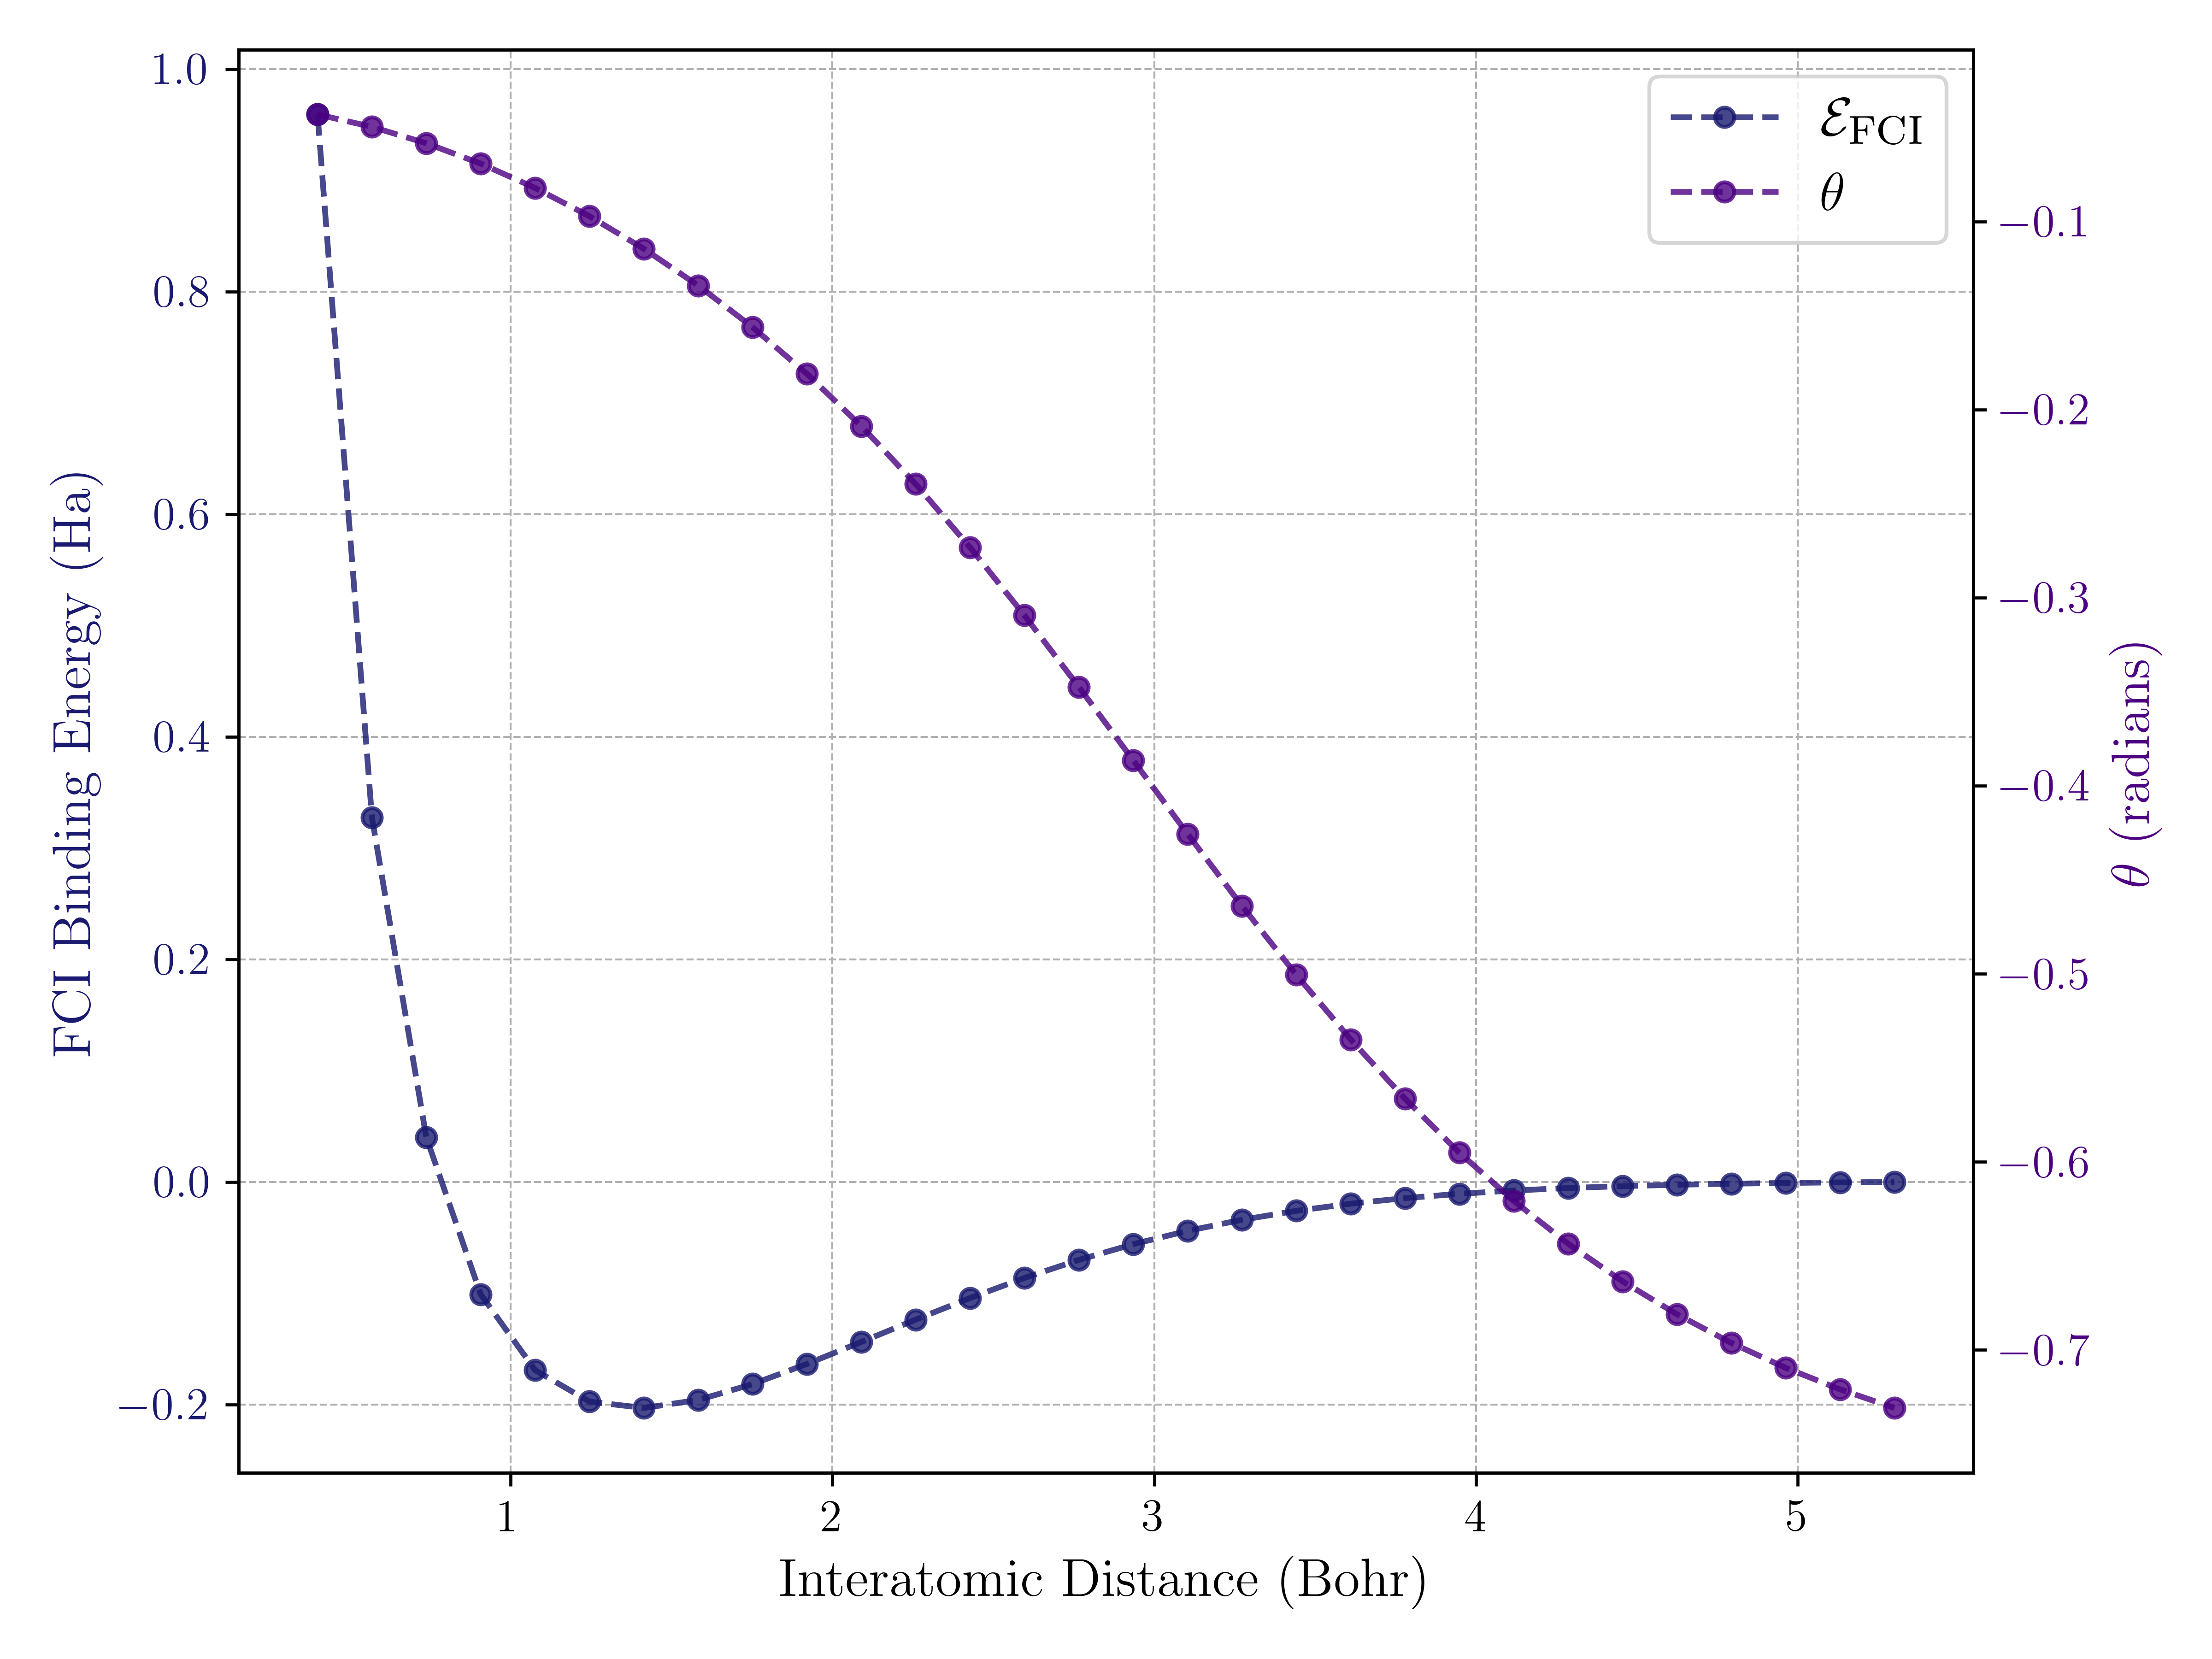
\includegraphics[width=0.5
                \textwidth]{figures/binding_theta.png}
                \caption{FCI binding energy $\mathcal E_\textsc{fci}$ and $\theta$ angle defining the ground state wavefunction of the H$_2$ dimer as a function of the interatomic distance.}
        \label{fig:binding_theta}
        \end{figure}

        \begin{figure*}[ht]
        \centering
            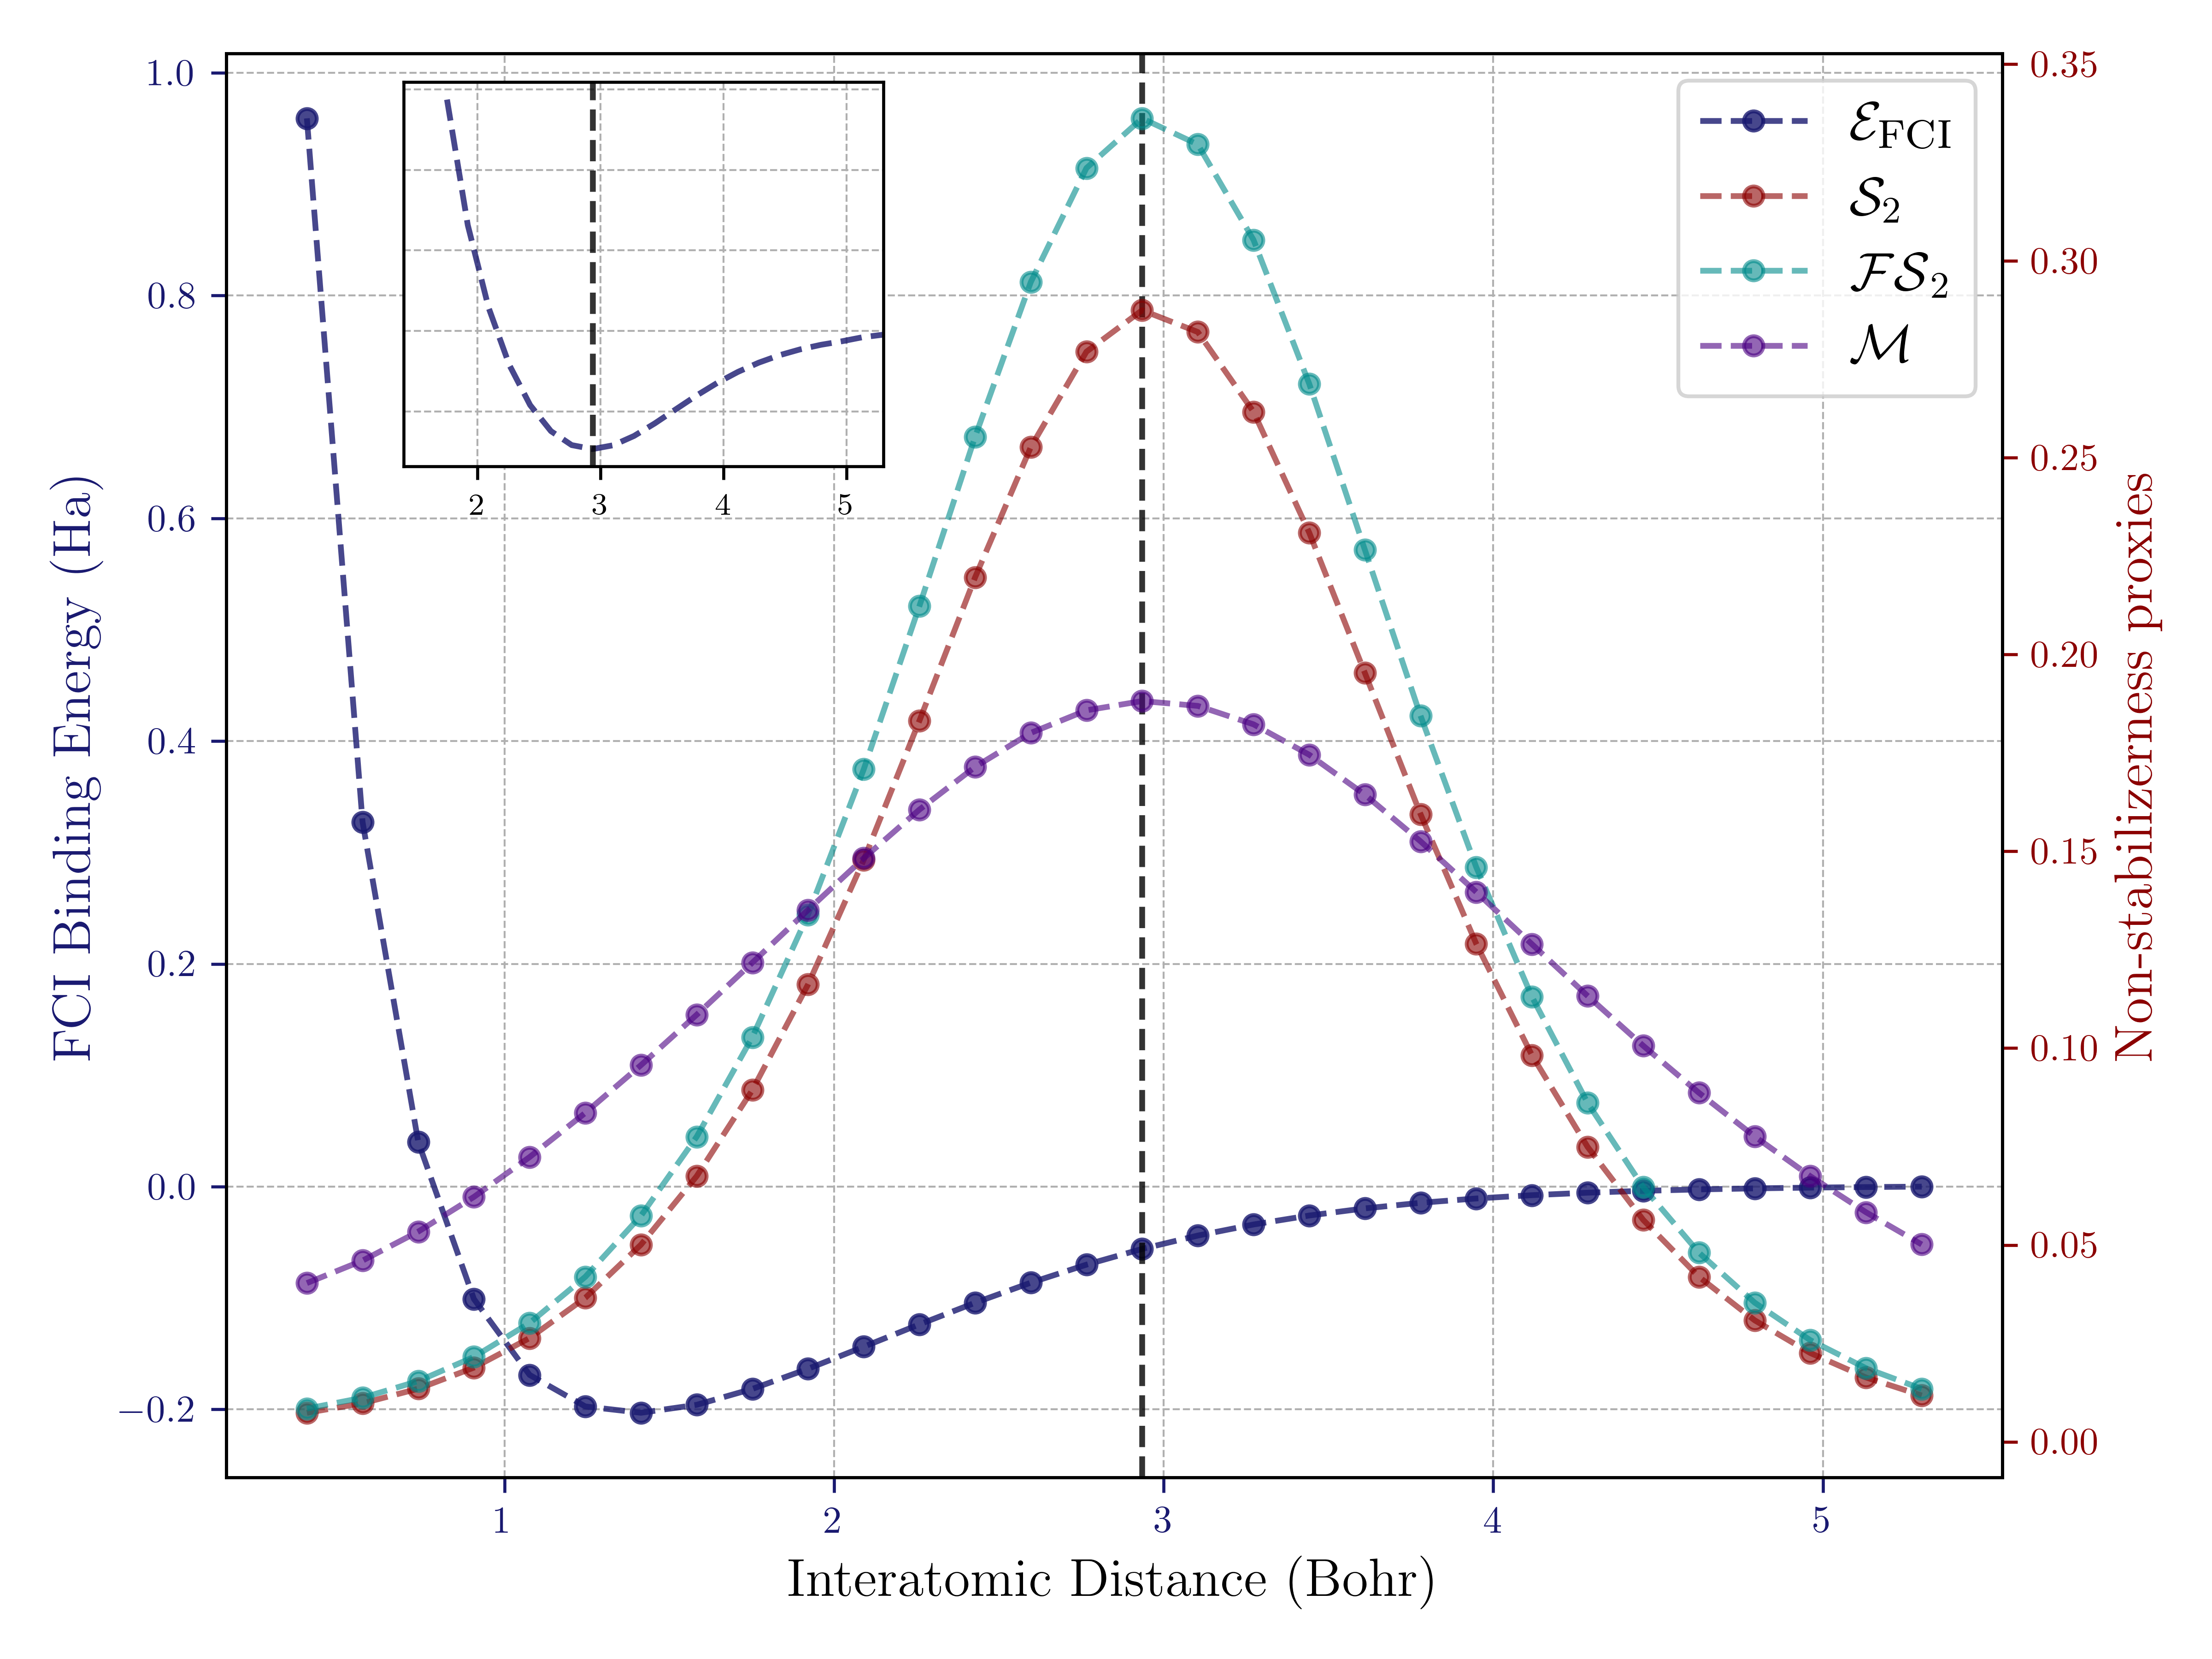
\includegraphics[width=1.0
            \textwidth]{figures/magic_vs_distance.png}
            \caption{Stabilizer Renyi entropy $\mathcal S_2$, filtered stabilizer Renyi entropy $\mathcal{FS}_2$, mana $\mathcal M$, and FCI binding energy $\mathcal E_\textsc{fci}$ as a function of the interatomic distance. These magic proxies exhibit a pronounced peak at the interatomic distance where the extrinsic curvature of the binding energy curve is maximal, as indicated by the vertical dashed line. The inset depicts the second derivative of the FCI binding energy, confirming the relation between the magic proxies and the curvature of the binding energy curve.}
        \label{fig:magic_vs_distance}
        \end{figure*}

    \subsection{Behavior of the Magic Proxies and physical interpretation}

        Let us define the extrinsic curvature of the binding energy curve as
        \begin{equation}
            \kappa(\ell) = \frac{\left|\mathcal E_\textsc{fci}''(\ell)\right|}{\left[1+\mathcal E_\textsc{fci}'(\ell)^2\right]^{3/2}},
        \end{equation}
        Let us denote by $\ell^\star$ the point of maximal extrinsic curvature of the binding energy curve $\ell^\star = \argmax_{\ell} \kappa(\ell)$.
        For each value of the interatomic distance $\ell$, we compute the fermionic Wigner function of the ground state and evaluate the magic proxies defined in the first Section of the paper. The reader will find in Fig.~\ref{fig:magic_vs_distance} the behavior of the stabilizer Renyi entropy $\mathcal S_2$ and the mana $\mathcal M$ as a function of the interatomic distance $\ell$.

        Our results reveal a striking phenomenon: as the hydrogen atoms approach each other, the magic proxies develop a pronounced peak precisely at the interatomic distance where the extrinsic curvature of the binding energy curve is maximal. This suggests that the bonding process is accompanied by a significant increase in non-stabilizerness, implying that the formation of a covalent bond requires the consumption of a large amount of non-Clifford operations.

        From the perspective of resource theories in quantum computation, a state with low magic is efficiently classically simulable, while high magic is a necessary ingredient for quantum computational speedup \cite{howard2014contextuality,Veitch2014Resource}. Thus, our analysis indicates that the H$_2$ bond formation is not only a chemical process but also a transformation that incurs a cost in terms of quantum computational resources.

        The observation of a magic peak coinciding with the maximal extrinsic curvature of the binding energy curve has profound implications. It suggests that the energetics of molecular bonding can be interpreted through the lens of quantum information theory: the system must “pay” a price in terms of magic to establish the correlated, entangled state necessary for a stable bond.

        Moreover, this interplay between chemical binding and quantum computational resources opens up several new avenues. For instance, one might ask whether the degree of non-stabilizerness correlates with chemical reactivity or catalytic efficiency. Similarly, in the context of quantum simulation, understanding how magic is generated and consumed during chemical reactions could inform the design of more efficient quantum algorithms for molecular modeling.

        Here, the angle $\theta$ adjusts continuously with $\ell$, reflecting the relative weight of two determinants. In regions where the determinants contribute comparably, the interference between them amplifies off‑diagonal correlations in the Majorana basis, leading to a more “spread out” fermionic Wigner function and, consequently, to a higher value of our magic proxies.

        From the standpoint of molecular physics and quantum chemistry, our results offer an intriguing reinterpretation of chemical bond formation:

        In the dissociation limit ($\ell\to\infty$), the hydrogen atoms are essentially isolated. The electronic wavefunction factorizes, leading to a state that is close to a product state. In such a regime, the fermionic correlations are minimal and the associated magic (or non‑stabilizerness) is low, consistent with the notion of a classically tractable system.

        At interatomic distances near $\ell^\star$, where the binding energy curve shows maximal extrinsic curvature, the wavefunction represents a delicate balance between the two determinants. This is the regime where the chemical bond is forming. The competition between the ionic and covalent contributions—and the ensuing cancellation in the ionic part—results in a highly correlated state. Our analysis shows that this is the very point at which the quantum state demands a larger number of non‑Clifford operations for its simulation, as reflected by the peak in magic proxies.

        The extrinsic curvature $\kappa$ is a geometric measure of the sensitivity of the binding energy with respect to interatomic distance. Its maximum marks a rapid change in the energy landscape—a signature of a transition in the electronic structure. This energetic reorganization is directly correlated with the rise in non‑stabilizerness, indicating that the very formation of the covalent bond is accompanied by an increase in the quantum complexity of the state.

        The confluence of these perspectives reinforces a remarkable insight: the process of chemical bond formation is not solely an energetic or structural rearrangement but is also accompanied by a non‑trivial transformation in the quantum informational character of the state. At large distances, the electrons are described by nearly independent, stabilizer‑like states, whereas in the bonding region the superposition of determinants—and the ensuing electron correlation—requires an injection of magic into the system. This observation opens a conceptual bridge between quantum resource theories and chemical reactivity, suggesting that the cost of forming a bond can be viewed through the lens of quantum computational resources.

\section{Outlook}

    While our study focuses on the simple hydrogen dimer, it would be instructive to extend this analysis to more complex molecules. The methodology we employed – combining \textit{ab initio} methods with quantum resource-theoretic measures – can be extended to other molecules and more sophisticated bases. One could, for instance, analyze the magic content in a stretched water molecule or in a transition metal dimer where multi-reference character is strong. We expect that systems requiring multi-reference descriptions will generally show nonzero mana. It would be enlightening to examine how mana scales with system size for a given chemical family: e.g., does adding more electrons in similar bonds increase the mana proportionally, or can mean-field capture more of it? Do peaks in magic proxies universally signal the formation of covalent bonds or reaction barriers? Investigating larger systems could also illuminate whether the degree of non‑stabilizerness correlates with chemical reactivity or catalytic efficiency.

    The observed interplay between electronic structure and quantum computational resources suggests that quantum simulations of chemistry could benefit from incorporating magic measures as diagnostic tools. In turn, these insights may lead to the design of more efficient quantum algorithms that adapt to the changing resource demands along reaction coordinates.

    Although magic is a computational resource concept, there may be indirect experimental signatures—such as changes in entanglement spectra or spectroscopic features—that correlate with the onset of high magic. Exploring these connections could provide a new experimental window into quantum correlations in chemical systems.

    Finally, our results hint at a broader framework where concepts from quantum information theory beyond pure entanglement entropy measures (like non‑stabilizerness) can serve as indicators of physical phenomena. This cross-disciplinary approach could pave the way for a unified understanding of complex quantum processes, blending the rigorous formalism of quantum computing with the rich phenomenology of chemical physics.

\vspace{1em}
\paragraph*{acknowledgments}

    The authors acknowledge funding via the FNR-CORE Grant ``BroadApp'' (FNR-CORE C20/MS/14769845) and ERC-AdG Grant ``FITMOL''.

\vspace{1em}
\paragraph*{Code and Data Availability}

    The reader will find an open source python code accompanying this paper at \esrgithub.

%\bibliographystyle{apsrev4-2}
\nocite{*}
\bibliography{bibliography}

\end{document}